\documentclass[compress, aspectratio=169]{beamer}

\usefonttheme{professionalfonts}

\usepackage{fontspec}
\usepackage{polyglossia}
\setmainlanguage{german}

\usepackage{microtype}

\usepackage{mathtools}
\usepackage[
  math-style=ISO,
  bold-style=ISO,
  nabla=upright,
  partial=upright,
]{unicode-math}

\usepackage[]{csquotes}
\usepackage[locale=DE,
            math-rm=\mathup,
            load-configurations=astronomy,
            per-mode=symbol-or-fraction,
          ]{siunitx}
\DeclareSIUnit{\year}{a}

\usepackage{graphicx}

\usepackage{tikz}
\usetikzlibrary{arrows}
\usetikzlibrary{arrows.meta}
\usetikzlibrary{shapes}

\usepackage{pgfplots}
\usepgfplotslibrary{polar}
\pgfplotsset{compat=1.12}

\newcommand\fullscreenimage[1]{{%
  \usebackgroundtemplate{%
    \includegraphics[
      width=\paperwidth,
      height=\paperheight,
  ]{#1}}
  \begin{frame}[plain]%
  \end{frame}%
}}


\usepackage{xfrac}


\usetheme{vertex}

\newcommand\SIQ[2]{\ensuremath{#1\mathrel{/}\si{#2}}}
\newcommand\PI{\ensuremath{\mathup{π}}}
\newcommand\kb{\ensuremath{k_\mathup{B}}}
\newcommand\TB{\ensuremath{T_\mathup{B}}}


\author{Maximilian Nöthe}
\date[21.5.2015]{Seminar Radioastronomie, TU Dortmund, 21.5.2015}
\title{Das Wasserstoffspektrum}
\subtitle{in der Radioastronomie}

\begin{document}
\maketitle

\section{Linien-Emission}
\begin{frame}{Einstein-Koeffizienten}
  \begin{columns}[T, onlytextwidth]%
    \begin{column}{0.5\textwidth}%
      \begin{tikzpicture}[
  scale=0.75,
  level/.style={very thick},
  photon/.style={-{Stealth[length=2mm]}, color=red!70!black, thick, decorate, decoration={snake, pre length=0.5mm, post length=1mm,}},
  connect/.style={dashed, very thick},
  ]
  \draw[level] (0,  0) node [left] {$E_2$} -- +(8, 0);
  \draw[level] (0, -2) node [left] {$E_1$} -- +(8, 0);
  \draw[photon] (2, 0) -- +(0,-2) node [below] {\normalcolor Emission} node[midway,left] {$A_{21}$};
  \draw[photon] (4,-2) -- +(0, 2) node [above] {\normalcolor Absortion} node[midway,left] {$B_{12}\bar{U}$};
  \draw[photon] (6, 0) -- +(0,-2) node [below] {\normalcolor stim.\ Emission} node[midway, right] {$B_{21}\bar{U}$};
  \draw[photon] (5,-1) -- +(0.95, 0);
\end{tikzpicture}
%
    \end{column}%
    \begin{column}{0.45\textwidth}%
      mittlere Energiedichte:
      \begin{equation*}
        \bar{U} = \frac{4\PI}{c} \bar{I},\quad\text{$\bar{I} =$ mittlere Intensität}
      \end{equation*}
      in statischem System:
      \begin{equation*}
        N_2 A_{21} + N_2 B_{21} \bar{U} = N_1 B_{12} \bar{U}
      \end{equation*}
      Mit $N_i =$ Anzahl Elektronen auf Energieniveau $E_i$
    \end{column}%
  \end{columns}%
\end{frame}

\begin{frame}{Wichtige Kenngrößen}
  \begin{block}{Brightness Temperature $T_\mathup{B}$}
    \begin{align*}%
      \TB &= \frac{c²}{2 \kb} \frac{1}{ν²} I_ν & 
      \TB &= \frac{h ν}{k_\mathup{B}}
             \frac{1}{\ln\!\left(
                \frac{8\PI h ν³}{c³\bar{U}} + 1
             \right)} \\
      &\text{(allgemein)} &  &\text{(Linienemission)}
    \end{align*}%
  \begin{itemize}
    \item Rayleigh–Jeans-Temperatur für gegebene Intensität $I_ν$
    \item verbreitetes Helligkeitsmaß in der Radioastronomie
  \end{itemize}
  \end{block}%
\end{frame}

\begin{frame}{Die \SI{21}{\centi\meter}-Linie}
  \begin{columns}[c, onlytextwidth]%
    \begin{column}{0.6\textwidth}%
      \begin{tikzpicture}[
    level/.style={very thick},
  photon/.style={-{Stealth[length=2mm]}, thick, decorate, decoration={snake, pre length=1mm, post length=2mm,}}, connect/.style={dashed, very thick},
  ]
  \draw[level] (0, 0) -- (+1.5, 0) node at (0, 0) [above] {$1^2S_{\sfrac{1}{2}}$};
  \draw[connect] (1.5, 0) -- +(1.5,  1);
  \draw[connect] (1.5, 0) -- +(1.5, -1);
  \draw[level] (3,  1) -- +(1.5, 0);
  \draw[level] (3, -1) -- +(1.5, 0);

  \draw[red!70!black, ->, thick] (3.75, 1) -- +(0, -2)
    node[right, midway] {$\increment E = \SI{5.9e-6}{\electronvolt}$};
  \draw[red!70!black, photon] (3.75, 0) -- + (-3, -2)
  node[below, align=left] {$λ = \SI{21.11}{\centi\meter}$ \\ $f = \SI{1420.406}{\mega\hertz}$};
  \node[] at (5,  1) {$\uparrow \quad \uparrow$};
  \node[] at (5, -1) {$\uparrow \quad \downarrow$};
  \node[] at (5,  1.5) {$\mathup{p}\quad\mathup{e}$};
\end{tikzpicture}

    \end{column}%
    \begin{column}{0.4\textwidth}%
      \begin{itemize}
        \item Hyperfeinstruktur-Übergang in neutralem H
        \item stark unterdrückt:
          \begin{gather*}
            A_{21} = \SI{2.869e-15}{\per\second} \\
            τ = \SI{1.1e7}{\year}
          \end{gather*}\vspace{-1.5\baselineskip}%
        \item Anregung durch Stöße im interstellarem Medium
      \end{itemize}
    \end{column}%
  \end{columns}%
\end{frame}

\section{Die \texorpdfstring{$\color{darkred}\SI{21}{\centi\meter}$}{21 cm}-Linie}
\subsection{Geschichte}
\begin{frame}{Geschichte}%
  \begin{columns}[c, onlytextwidth]%
    \column{0.15\textwidth}%
      \centering
      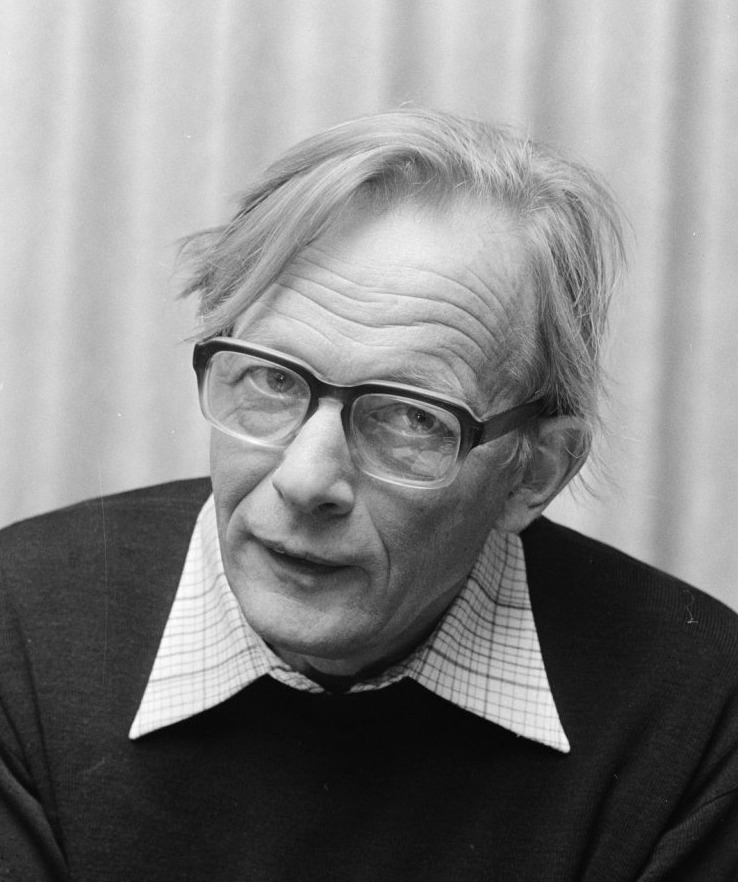
\includegraphics[width=\linewidth]{./images/Hendrik_vanDeHulst.jpg}
      \newline H. v.\,d. Hulst
    \column{0.8\textwidth}%
      \begin{description}[Hendrik van de Hulst]
        \item[Hendrik van de Hulst] Holländischer Astronom \& Mathematiker
        \item[1944] Vorhersage der \SI{21}{\centi\meter}-Linie
        \item[später] Mitarbeit bei der Kartographie der Milchstraße
      \end{description}
  \end{columns}%
  \vfill
  \begin{columns}[c, onlytextwidth]%
    \column{0.15\textwidth}%
      \centering
      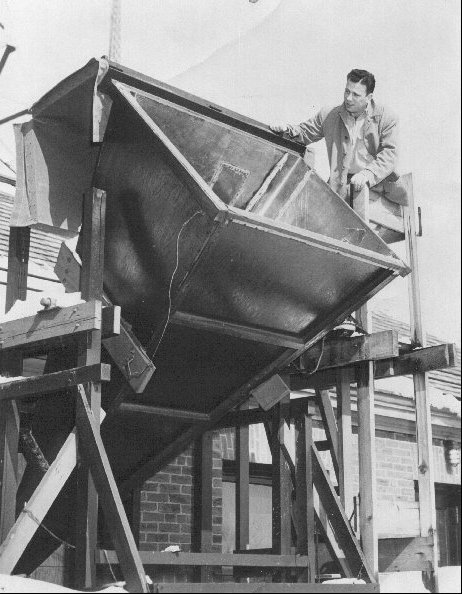
\includegraphics[width=\linewidth]{./images/ewenhorn.jpg}%
      \newline H.~Ewen
    \column{0.65\textwidth}%
      \begin{description}[1951]
        \item[1951] Entdeckung durch Edward Purcell \& Harold Ewen\\
                    an der Harvard University
      \end{description}
    \column{0.15\textwidth}%
      \centering
      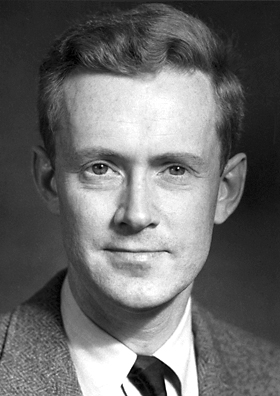
\includegraphics[width=\linewidth]{./images/Edward_Mills_Purcell.jpg}%
      \newline E.~Purcell
  \end{columns}%
\end{frame}
\subsection{Entstehung}
\begin{frame}{Die \SI{21}{\centi\meter}-Linie}
  \begin{columns}[c, onlytextwidth]%
    \begin{column}{0.6\textwidth}%
      \begin{tikzpicture}[
    level/.style={very thick},
  photon/.style={-{Stealth[length=2mm]}, thick, decorate, decoration={snake, pre length=1mm, post length=2mm,}}, connect/.style={dashed, very thick},
  ]
  \draw[level] (0, 0) -- (+1.5, 0) node at (0, 0) [above] {$1^2S_{\sfrac{1}{2}}$};
  \draw[connect] (1.5, 0) -- +(1.5,  1);
  \draw[connect] (1.5, 0) -- +(1.5, -1);
  \draw[level] (3,  1) -- +(1.5, 0);
  \draw[level] (3, -1) -- +(1.5, 0);

  \draw[red!70!black, ->, thick] (3.75, 1) -- +(0, -2)
    node[right, midway] {$\increment E = \SI{5.9e-6}{\electronvolt}$};
  \draw[red!70!black, photon] (3.75, 0) -- + (-3, -2)
  node[below, align=left] {$λ = \SI{21.11}{\centi\meter}$ \\ $f = \SI{1420.406}{\mega\hertz}$};
  \node[] at (5,  1) {$\uparrow \quad \uparrow$};
  \node[] at (5, -1) {$\uparrow \quad \downarrow$};
  \node[] at (5,  1.5) {$\mathup{p}\quad\mathup{e}$};
\end{tikzpicture}

    \end{column}%
    \begin{column}{0.4\textwidth}%
      \begin{itemize}
        \item Hyperfeinstruktur-Übergang in neutralem H
        \item stark unterdrückt:
          \begin{gather*}
            A_{21} = \SI{2.869e-15}{\per\second} \\
            τ = \SI{1.1e7}{\year}
          \end{gather*}\vspace{-1.5\baselineskip}%
        \item Anregung durch Stöße im interstellarem Medium
      \end{itemize}
    \end{column}%
  \end{columns}%
\end{frame}

\subsection{Messungen}
\begin{frame}{Die \SI{21}{\centi\meter}-Linie – Vermessung der Milchstraße}%
  \begin{columns}[c, onlytextwidth]
    \begin{column}{0.47\textwidth}%
      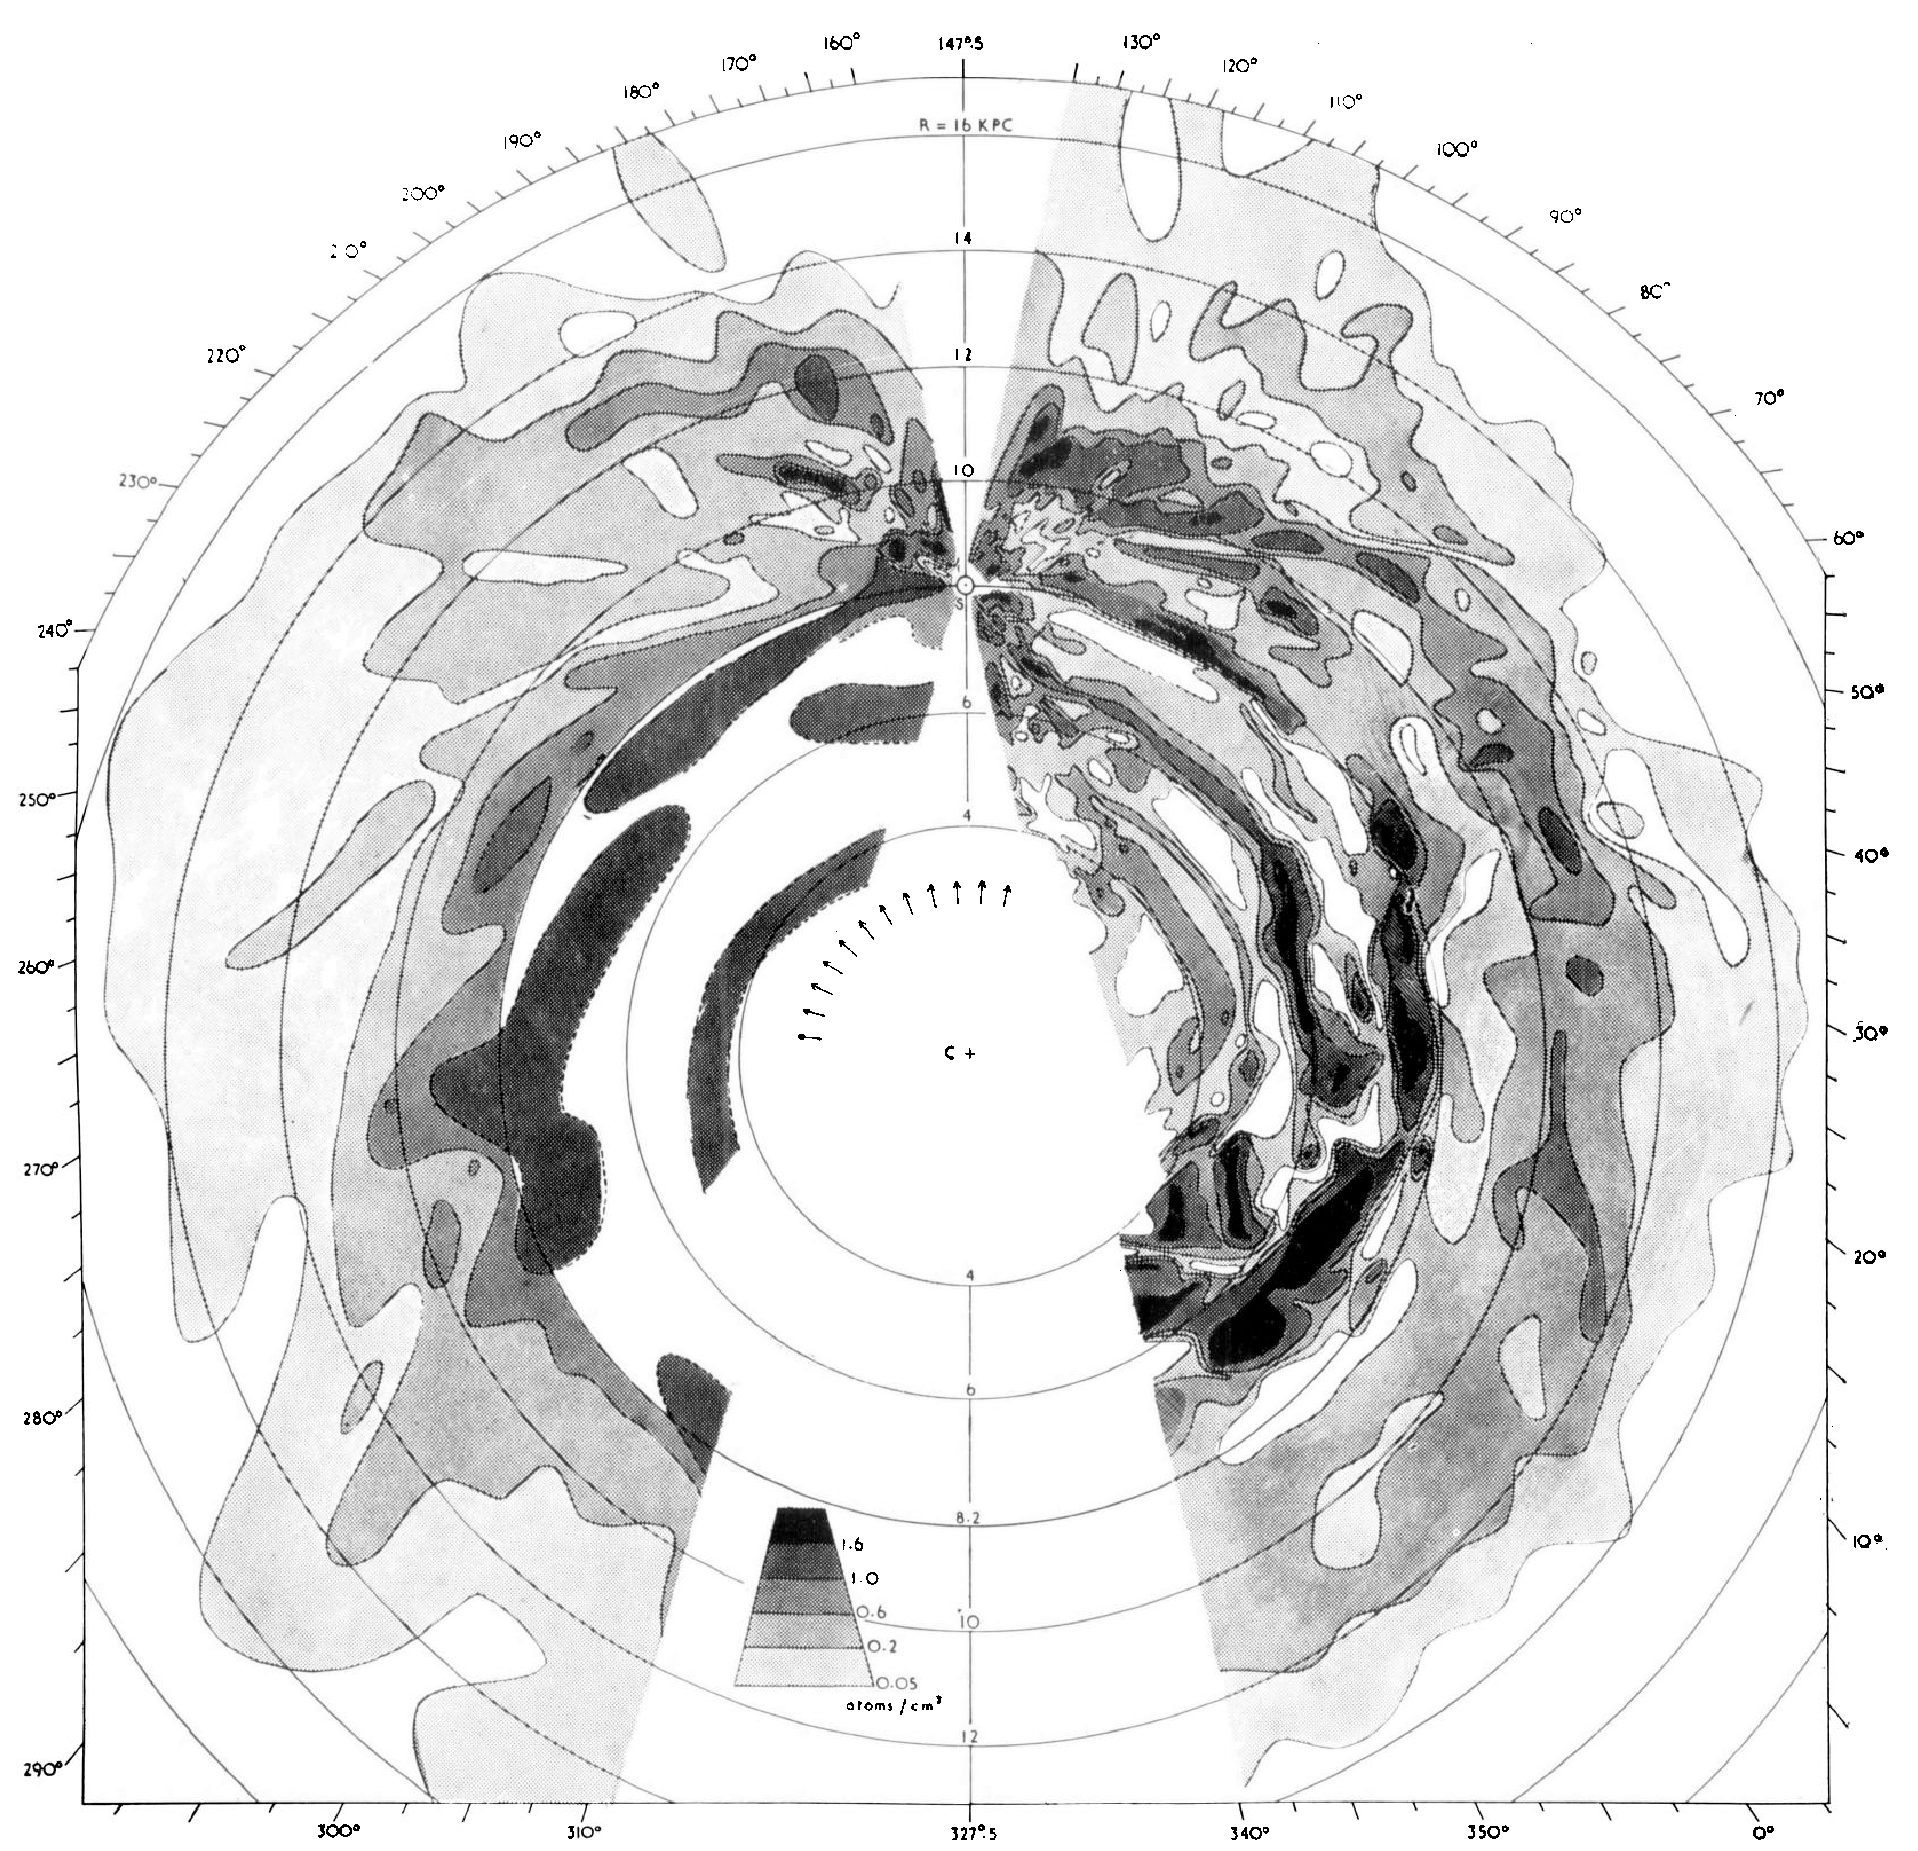
\includegraphics[width=\textwidth, angle=180]{./images/original_map.png}%
    \end{column}%
    \begin{column}{0.47\textwidth}%
      \begin{description}[Messung]
        \item[1958] Veröffentlichung der ersten \enquote{Karte} der Milchstraße
        \item[Autoren] J. H. Oort, F. J. Kerr und G. Westerhout
        \item[Messung] \SI{7.5}{\meter}-Teleskop (Leiden) \&  \SI{11}{\meter}-Teleskop (Sidney)
      \end{description}

      \begin{center}
      \parbox{0.85\linewidth}{\enquote{The \SI{21}{\centi\meter} oberservations brought about a revolution in the study of galactic structure}}
      \end{center}
    \end{column}%
  \end{columns}
\end{frame}

\begin{frame}{Messprinzip}
  \begin{columns}[c, onlytextwidth]
    \begin{column}{0.5\textwidth}
      \newcommand{\viewangle}{19.471220634490692}
\newcommand{\cloudangleA}{79.5}
\newcommand{\cloudangleB}{-40.7}
\begin{tikzpicture}[
    hydrogen/.style={fill, anchor=center, black!20,
    cloud, draw, cloud puffs=11, minimum size=0.5cm,
    cloud puff arc=120, aspect=3, inner sep=0em}
]
  \draw[thin] (0, 0) circle [radius = 1];
  \draw[thin] (0, 0) circle [radius = 2];
  \draw[thin] (0, 0) circle [radius = 3];
  \node[hydrogen]  at (\viewangle:1cm) {};
  \node[hydrogen]  at (\cloudangleA:2cm) {};
  \node[hydrogen]  at (\cloudangleB:2cm) {};
  \draw[darkred, ->, dashed, thick] (0, 3) -- +(-90+\viewangle:6.5cm);
  \filldraw (0, 0) circle [radius=2pt];
  \filldraw (0, 3) circle [radius=2pt] node[above] {Sonnensystem};
  \draw[->, thick, blue] (\cloudangleA:2cm) -- +(\cloudangleA-90:1cm) node[above, midway] {$v_1$};
  \draw[->, thick, blue] (\cloudangleA:2cm) -- +(\viewangle-90:0.55cm);
  \draw[->, thick, green] (\viewangle:1cm) -- +(-90+\viewangle:1.2cm) node[right, midway] {$v_2$};
  \draw[->, thick, red] (\cloudangleB:2cm) -- +(\cloudangleB-90:1cm) node[anchor=south east, midway] {$v_3$};
  \draw[->, thick, red] (\cloudangleB:2cm) -- +(\viewangle-90:0.49cm);
\end{tikzpicture}

    \end{column}
    \begin{column}{0.5\textwidth}
      \begin{tikzpicture}%
        \begin{axis}[%
            xmin=21.1,
            xmax=21.13,
            ymin=0,
            % ymax=120,
            width=\linewidth-12.05pt,
            xlabel={\SIQ{λ}{\centi\meter}},
            ylabel={$I$ / a.\,u.},
            extra x ticks={21.10611405413},
            extra x tick labels={$\mathrm{H}$},
          ]%
          \addplot[
            green,
            domain=21.1:21.13,
            samples=201,
          ]{0.6*exp(-0.5*(x-21.122)^2/(0.002^2))/(sqrt(2*pi*0.002^2))};
          \addplot[
            red,
            domain=21.09:21.12,
            samples=201,
          ]{0.6*exp(-0.5*(x-21.112)^2/(0.002^2))/(sqrt(2*pi*0.002^2))};
          \addplot[
            blue,
            domain=21.09:21.12,
            samples=201,
          ]{0.6*exp(-0.5*(x-21.110)^2/(0.002^2))/(sqrt(2*pi*0.002^2))};
        \end{axis}%
      \end{tikzpicture}%
    \end{column}
  \end{columns}
\end{frame}

\begin{frame}{Messprinzip}
  \begin{columns}[c, onlytextwidth]
    \begin{column}{0.5\textwidth}
      \newcommand{\viewangle}{19.471220634490692}
\begin{tikzpicture}
  \draw[thin] (0, 0) circle [radius = 1];
  \draw[thin] (0, 0) circle [radius = 2];
  \draw[thin] (0, 0) circle [radius = 3];
  \filldraw[darkred!30] (0, 3) -- (0, 2.3) arc [start angle=270, end angle=270+\viewangle, radius=0.7cm] -- cycle;
  \node[fill, anchor=center, black!20,
    cloud, draw, cloud puffs=11, minimum size=0.5cm,
    cloud puff arc=120, aspect=3, inner sep=0em]  at (\viewangle:1cm) {};
  \draw[darkred, ->, dashed, thick] (0, 3) -- +(-90+\viewangle:6.5cm);
  \draw (0, 0) -- + (0, 3) node[midway,left] {$R_0$};
  \draw (0, 0) -- (\viewangle:1cm) node[midway,below] {$R$};
  \filldraw (0, 0) circle [radius=2pt];
  \filldraw (0, 3) circle [radius=2pt] node[above] {Sonnensystem};
  \draw[->, thick] (0, 3) -- + (1, 0) node[below, right] {$v_0$};
  \draw[->, thick] (0, 3) -- + (\viewangle - 90:0.333);
  \draw[->, thick] (\viewangle:1cm) -- +(-90+\viewangle:1cm) node[right, midway] {$v$};
  \node[left] at (0, 2.65) {$γ$};
\end{tikzpicture}

    \end{column}
    \begin{column}{0.5\textwidth}
      \begin{enumerate}
        \item Messung der Doppler-Verschiebung der \SI{21}{\centi\meter}-Linie
          in eine Richtung
        \item Berechne für $v_{\max}$ = maximale Geschwindigkeit:
          \belowdisplayskip=0ex
          \begin{align*}
            R &= R_0 \cdot \sin{γ} \\
            v &= v_{\max} + v_0 \cdot \sin{γ} 
          \end{align*}
        \item Für Milchstraße:
          \begin{align*}
            v_0 = \SI{220}{\kilo\meter\per\second} \\
          R_0 = \SI{8.5}{\kilo pc}
          \end{align*}
      \end{enumerate}
    \end{column}
  \end{columns}
\end{frame}

\begin{frame}{Ermittlung der Rotationskurve}
  \begin{itemize}
    \item Tangential Methode mit H\textsc{I}
      \begin{itemize}
        \item Messung für viele galaktische Längen $l$
        \item Ermittlung von $v_{\max}$, $R$, $v$
        \item aber: vergleichsweise hohe Unsicherheiten \cite{rotation_curve}
      \end{itemize}
    \item Stattdessen kombinierte Analyse von CO, H\textsc{I} und H\textsc{II} Linien
  \end{itemize}
\end{frame}


\begin{frame}{LAB-Messung}
  Leiden/Dwingeloo – Argentinien – Bonn \cite{lab-kalberla}
  \begin{description}[Ortsauflösung]
    \item[2005] Veröffentlichung der Daten von zwei Teleskopen für den ganzen Himmel
    \item[1989--1993] \SI{30}{\meter}-Teleskop Argentinien
    \item[1994--2000] \SI{25}{\meter}-Teleskop Dwingeloo
    \item[Bonn] Zusammenfassung und Kalibrierung
    \item[Ortsauflösung] \SI{0.5}{\degree}
    \item[$\textcolor{darkred}{v}$-Auflösung] \SI{1.3}{\kilo\meter\per\second}
    \item[$\textcolor{darkred}{\TB}$-Auflösung] \SI{0.07}{\kelvin}
  \end{description}
  Frei zugänglicher Datensatz $\TB(l,b,v)$ mit $\approx \num{2e6}$ Datenpunkten
\end{frame}


\begin{frame}{Die \SI{21}{\centi\meter}-Linie – Vermessung der Milchstraße}%
  \begin{columns}[c, onlytextwidth]%
    \begin{column}{0.47\textwidth}%
      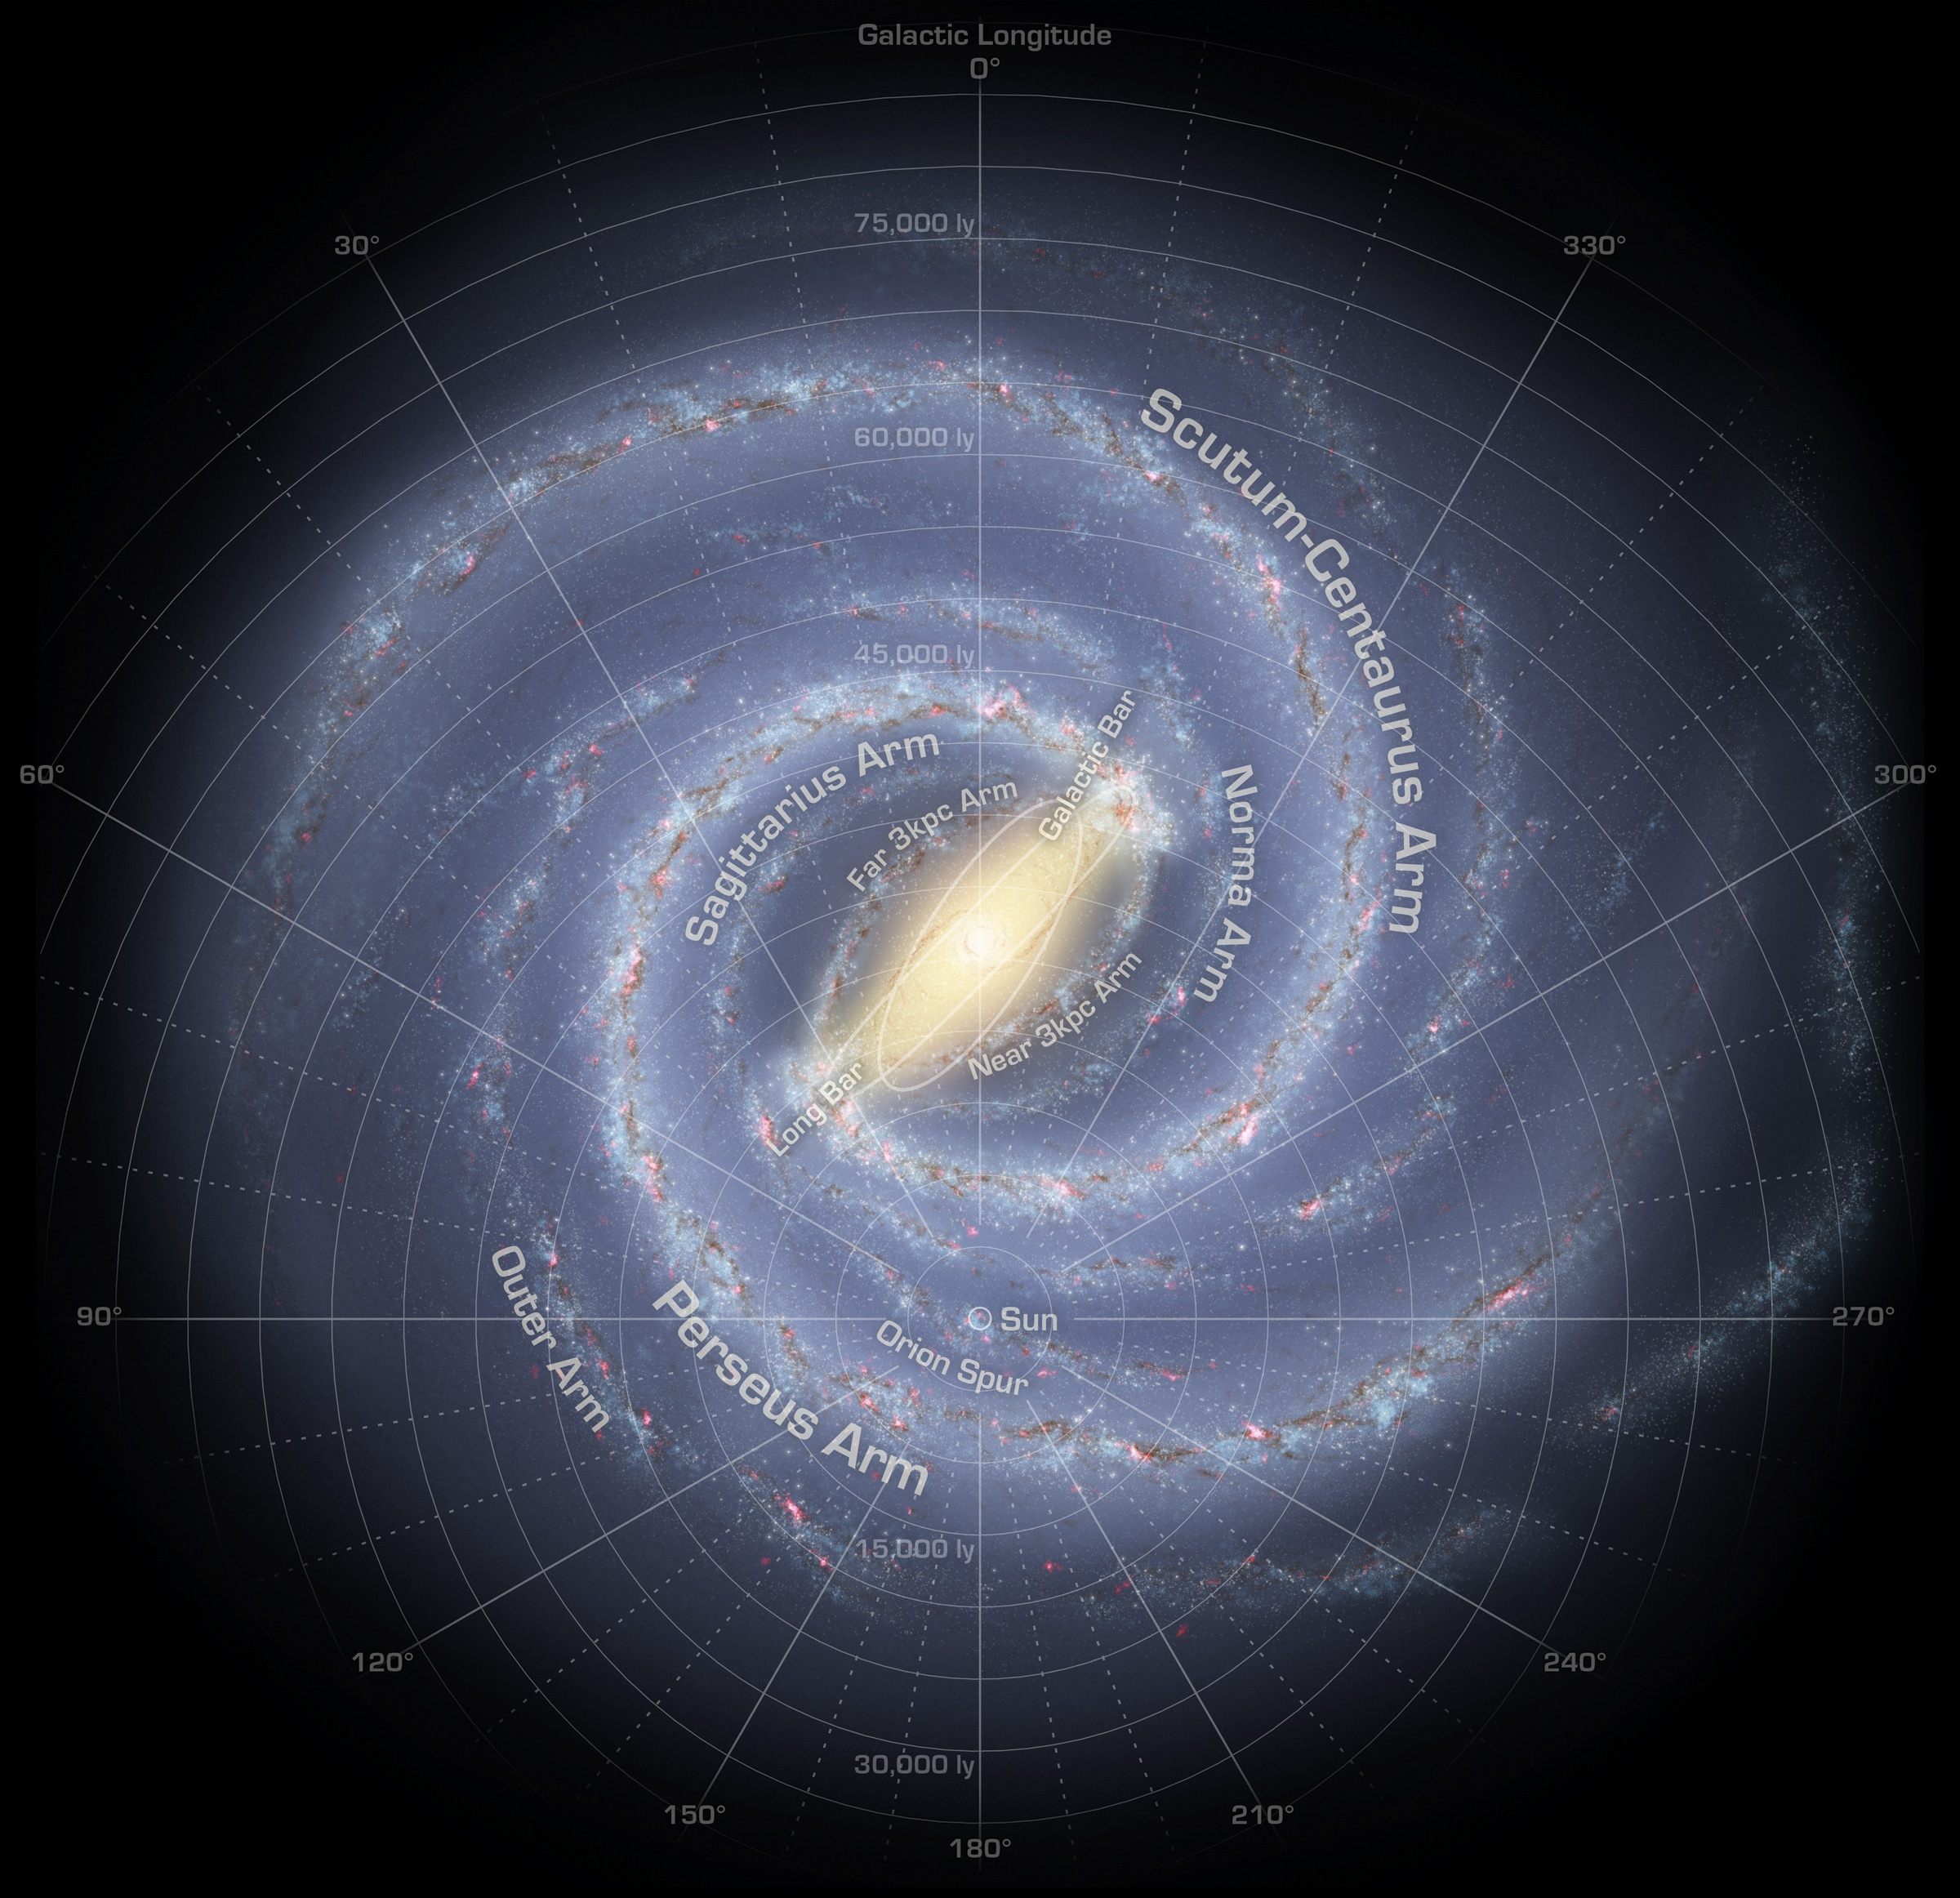
\includegraphics[width=\linewidth]{images/milkyway_structure_big_crop.jpeg}%
      \begin{tikzpicture}[overlay, remember picture, shift={(current page.center)}]%
        \only<1>{\draw[red!70!black, thick, o->] (-3.753, -1.41) -- +(65:4.5);}%
        \only<2>{\draw[red!70!black, thick, o->] (-3.819, -1.32) -- +(0:4.5);}%
      \end{tikzpicture}%
    \end{column}%
    \begin{column}{0.47\textwidth}%
      \begin{tikzpicture}%
        \begin{axis}[%
            title={$\TB$ für $l=\only<1>{\SI{335}{\degree}}\only<2>{\SI{270}{\degree}}$, \cite{lab-profile}},
            xmin=21.09,
            xmax=21.12,
            ymin=-10,
            ymax=120,
            width=0.93\linewidth,
            xlabel={\SIQ{λ}{\centi\meter}},
            ylabel={$\SIQ{\TB}{\kelvin}$},
            extra x ticks={21.10611405413},
            extra x tick labels={$\mathrm{H}$},
          ]%
          \only<1>{%
            \addplot[red!70!black] table[x index=3, y index=1]{./data/radial_velocity_l335.txt};%
          }
          \only<2>{%
          \addplot[red!70!black] table[x index=3, y index=1]{./data/radial_velocity_l270.txt};%
          }
        \end{axis}%
      \end{tikzpicture}%
    \end{column}%
  \end{columns}%
\end{frame}

\fullscreenimage[\cite{lab-survey}]{images/lab_survey.jpg}

\section{Messung am Stockert}
\begin{frame}{Messung am Stockert}
  \begin{columns}[c, onlytextwidth]
    \begin{column}{0.4\textwidth}
      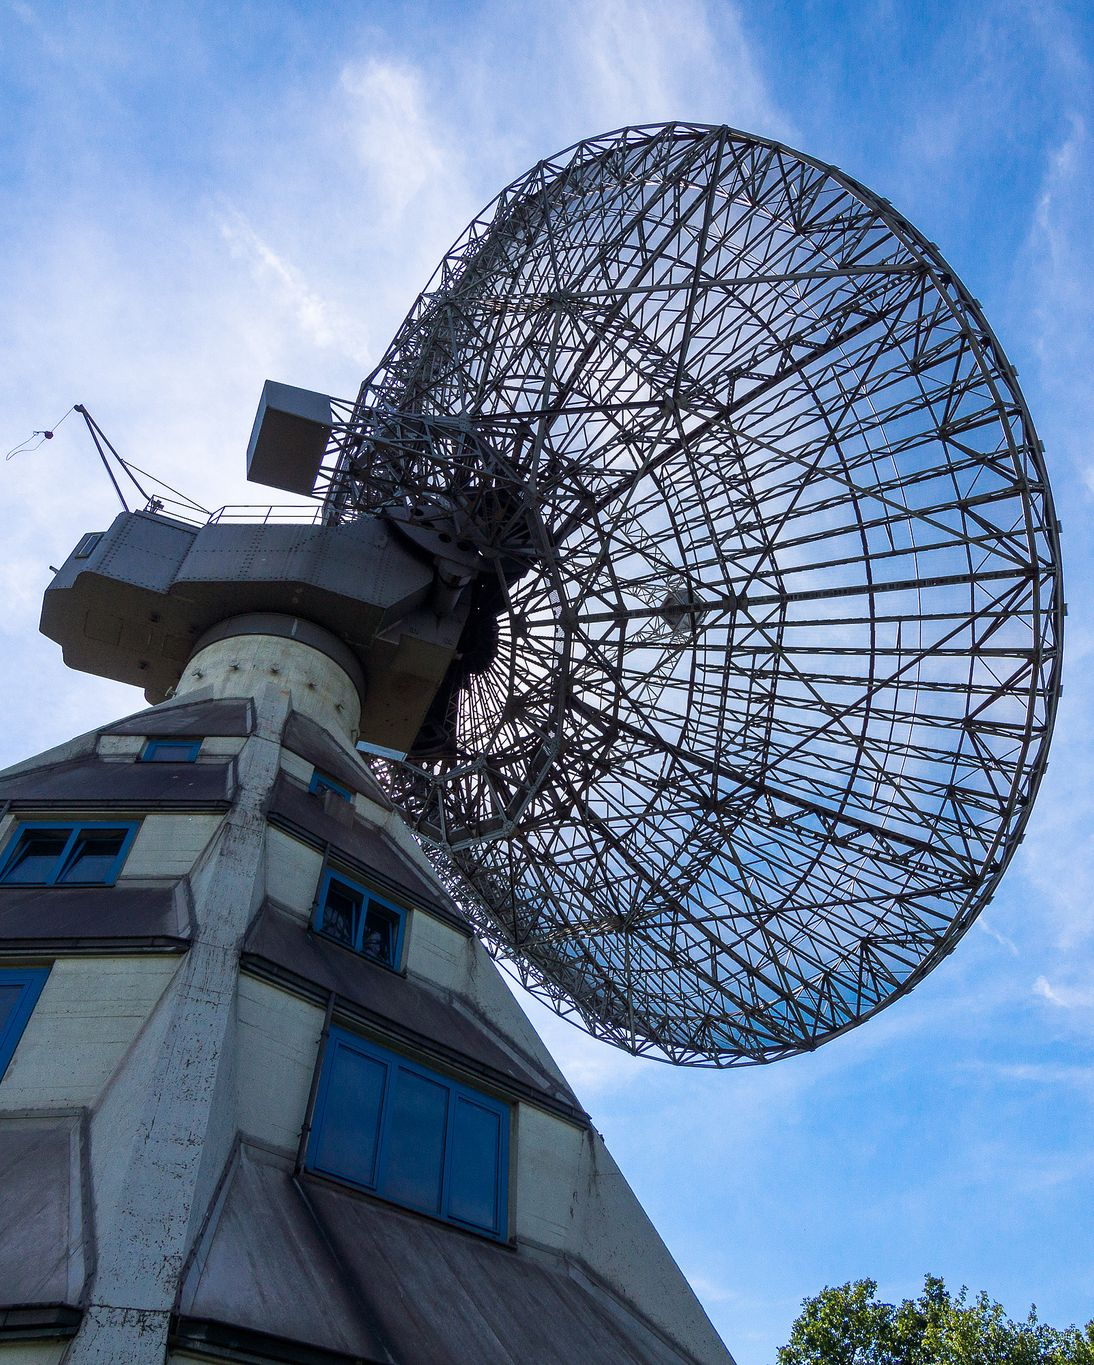
\includegraphics[width=\linewidth]{images/stockert_crop.jpg}
    \end{column}
    \begin{column}{0.55\textwidth}
      \begin{description}[Durchmesser]
        \item[Baujahr] 1956
        \item[Durchmesser] \SI{25}{\meter}
        \item[Auflösung]  \SI{0.5}{\degree} FWHM für $λ = \SI{21}{\centi\meter}$
        \item[Messung] Aufnahme von Spektren für verschiedene galaktische Längen
      \end{description}
    \end{column}
  \end{columns}
\end{frame}

\begin{frame}{Sichtbarkeit der Milchstraße}
  \begin{columns}[c, onlytextwidth]
    \begin{column}{0.65\textwidth}
      \begin{description}[15.6.2015]
        \item[1.6.2015] Arme in Zentrumsnähe ab ca. 20:30 Uhr \\
          Milchstraßen-Zentrum ca.\  22 – 4 Uhr
        \item[15.6.2015] Alle Zeiten ca.\ 30 Minuten früher
      \end{description}
    \end{column}
    \begin{column}{0.3\textwidth}
      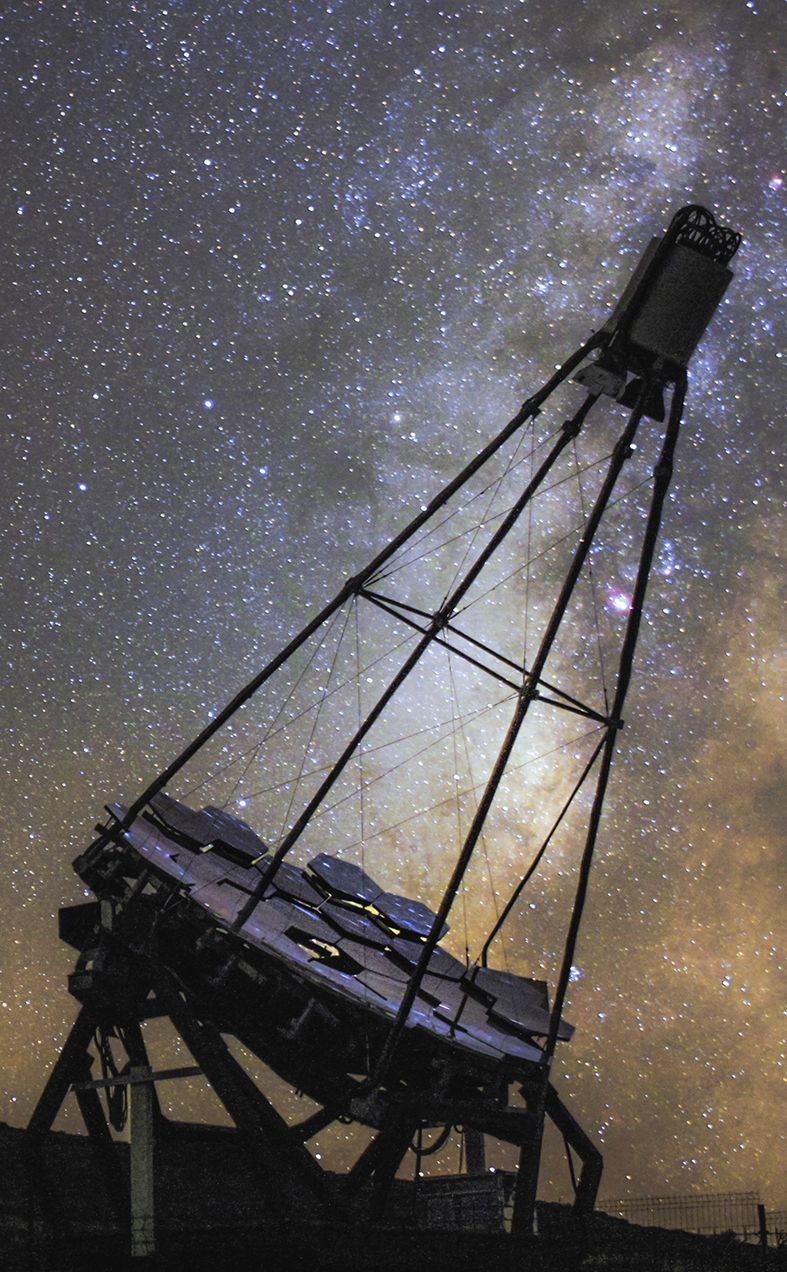
\includegraphics[width=\linewidth]{images/fact_crop.jpg}
    \end{column}
  \end{columns}
\end{frame}

\fullscreenimage[\color{darkred}1.6. 22:37 Uhr]{images/stellarium_20150601.jpg}

\section{HI in anderen Galaxien}
\begin{frame}[plain,t]{THINGS – extragalaktische \SI{21}{\centi\meter}-Linien}

  The H\textsc{I} Nearby Galaxy Survey – Very Large Array: 

  \begin{columns}[c, onlytextwidth]
    \begin{column}{0.4\textwidth}
      \begin{description}[Teleskope]
        \item[Ort] New Mexico, USA
        \item[Teleskope] 27 Stück \\
          \SI{25}{\meter} Durchmesser
      \end{description}
    \end{column}
    \begin{column}{0.55\textwidth}
      \begin{description}[Messdauer]
        \item[Auflösung] \SI{7}{\arcsecond} bzw. \SI{5}{\kilo\meter\per\second}
        \item[Messung] 34 Objekte zwischen  \num{3} und \SI{15}{\mega pc}
        \item[Messdauer] $> \SI{500}{\hour}$
      \end{description}
    \end{column}
  \end{columns}
  
  
  \begin{tikzpicture}[remember picture, overlay, shift=(current page.south west)]
    \node[anchor=south] at (0.5\paperwidth, -0.4) {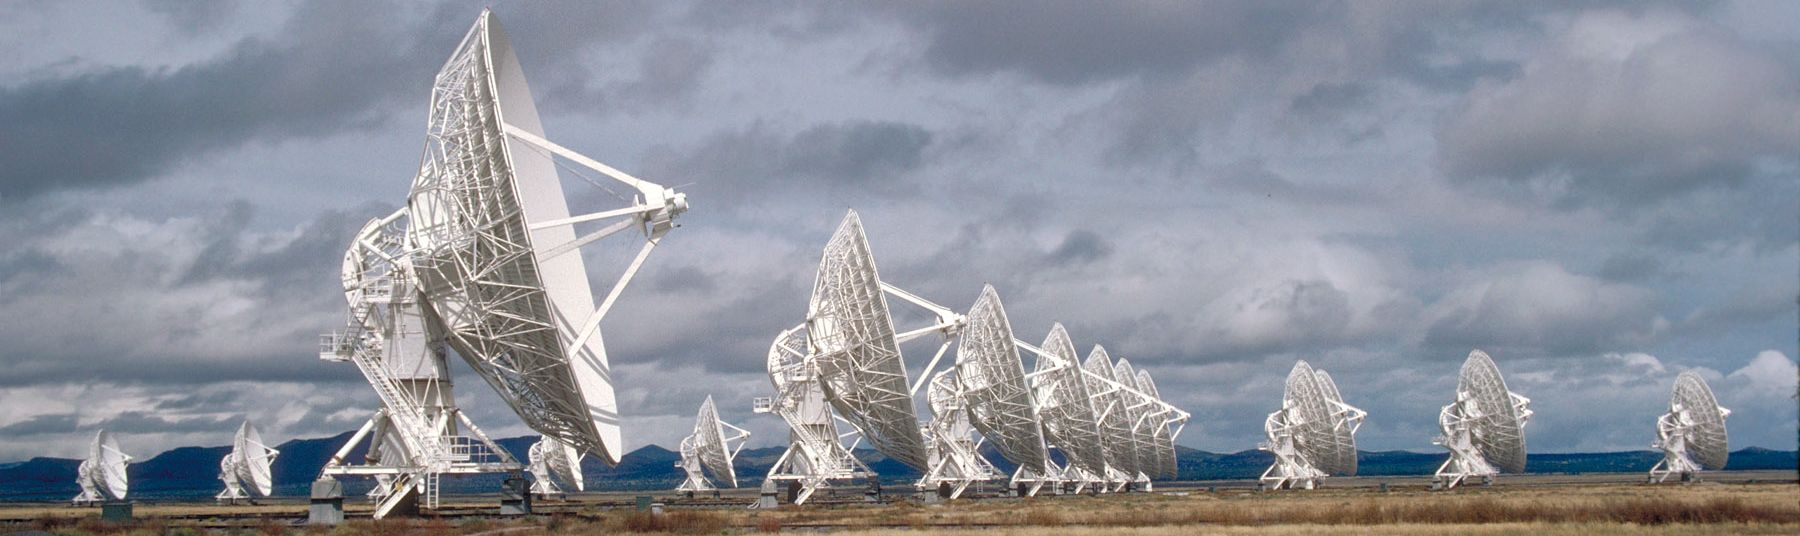
\includegraphics[width=\paperwidth]{images/vla_crop.jpg}};
  \end{tikzpicture}
\end{frame}

\fullscreenimage[\cite{things_galaxies}]{./images/things_galaxies.jpg}
\fullscreenimage[\cite{things_all}]{./images/things.png}

\end{document}
